\chapter{Diseño e implementación} % Main chapter title

\label{Chapter3} % Change X to a consecutive number; for referencing this chapter elsewhere, use \ref{ChapterX}

%----------------------------------------------------------------------------------------
Este capítulo brinda una explicación detallada del proceso de implementación de los algoritmos de detección facial, diseño de firmware y la integración de los servicios en la nube con el prototipo de pruebas.
%----------------------------------------------------------------------------------------


\definecolor{mygreen}{rgb}{0,0.6,0}
\definecolor{mygray}{rgb}{0.5,0.5,0.5}
\definecolor{mymauve}{rgb}{0.58,0,0.82}

%%%%%%%%%%%%%%%%%%%%%%%%%%%%%%%%%%%%%%%%%%%%%%%%%%%%%%%%%%%%%%%%%%%%%%%%%%%%%
% parámetros para configurar el formato del código en los entornos lstlisting
%%%%%%%%%%%%%%%%%%%%%%%%%%%%%%%%%%%%%%%%%%%%%%%%%%%%%%%%%%%%%%%%%%%%%%%%%%%%%
\lstset{ %
  backgroundcolor=\color{white},   % choose the background color; you must add \usepackage{color} or \usepackage{xcolor}
  basicstyle=\footnotesize,        % the size of the fonts that are used for the code
  breakatwhitespace=false,         % sets if automatic breaks should only happen at whitespace
  breaklines=true,                 % sets automatic line breaking
  captionpos=b,                    % sets the caption-position to bottom
  commentstyle=\color{mygreen},    % comment style
  deletekeywords={...},            % if you want to delete keywords from the given language
  %escapeinside={\%*}{*)},          % if you want to add LaTeX within your code
  %extendedchars=true,              % lets you use non-ASCII characters; for 8-bits encodings only, does not work with UTF-8
  %frame=single,	                % adds a frame around the code
  keepspaces=true,                 % keeps spaces in text, useful for keeping indentation of code (possibly needs columns=flexible)
  keywordstyle=\color{blue},       % keyword style
  language=[ANSI]C,                % the language of the code
  %otherkeywords={*,...},           % if you want to add more keywords to the set
  numbers=left,                    % where to put the line-numbers; possible values are (none, left, right)
  numbersep=5pt,                   % how far the line-numbers are from the code
  numberstyle=\tiny\color{mygray}, % the style that is used for the line-numbers
  rulecolor=\color{black},         % if not set, the frame-color may be changed on line-breaks within not-black text (e.g. comments (green here))
  showspaces=false,                % show spaces everywhere adding particular underscores; it overrides 'showstringspaces'
  showstringspaces=false,          % underline spaces within strings only
  showtabs=false,                  % show tabs within strings adding particular underscores
  stepnumber=1,                    % the step between two line-numbers. If it's 1, each line will be numbered
  stringstyle=\color{mymauve},     % string literal style
  tabsize=2,	                   % sets default tabsize to 2 spaces
  title=\lstname,                  % show the filename of files included with \lstinputlisting; also try caption instead of title
  morecomment=[s]{/*}{*/}
}

%----------------------------------------------------------------------------------------
\section{Detección facial con TensorFlow y TensorFlow Lite}
\label{section3_1}
Como se explicó en el capítulo \ref{Chapter1}, el objetivo principal de este trabajo es detectar rostros humanos con ayuda de algoritmos de AI. Para esto se deben obtener imágenes digitales con ayuda de una cámara, procesarlas y utilizarlas como entrada de una red de modelos de DL capaces de realizar la tarea de detección facial. Esta red de modelos fue descrita en el capítulo \ref{Chapter2} y se denomina MTCNN.

Para implementar MTCNN adecuadamente no basta con alimentar P-Net con las imágenes obtenidas por la cámara, R-Net con las ventanas candidatas de P-Net y O-Net con las ventanas candidatas de R-Net. Los datos de entrada de cada uno de los modelos de MTCNN deben ser procesados para conseguir el mejor resultado posible, como se muestra en el diagrama de la figura \ref{fig:mtcnn_npipe}.

\begin{figure}[h]
	\centering
	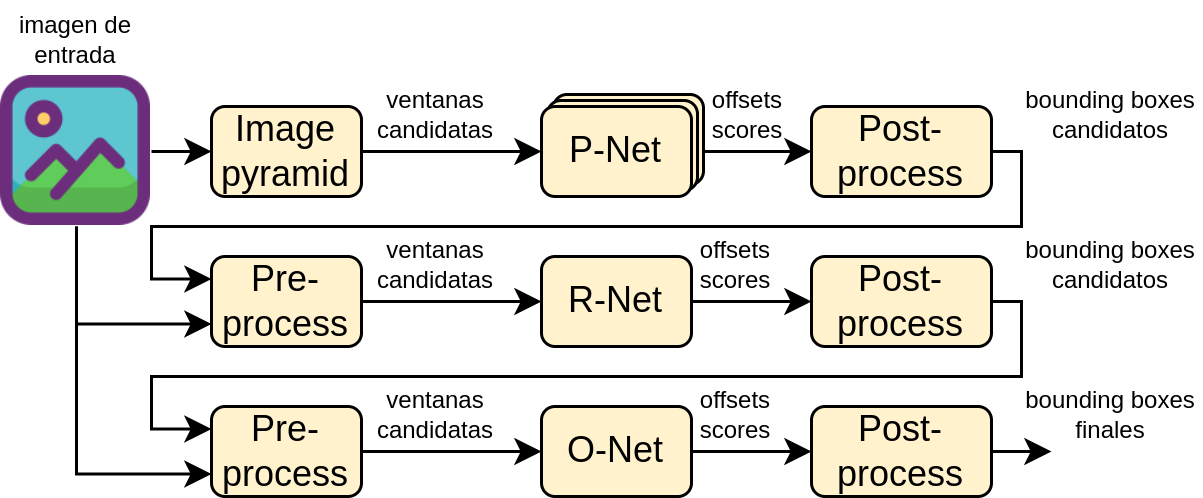
\includegraphics[scale=0.3]{./Figures/mtcnn_npipe.png}
	\caption{\textit{Pipeline} detallado de MTCNN.}
	\label{fig:mtcnn_npipe}
\end{figure}

El diagrama de la figura \ref{fig:mtcnn_npipe} muestra el \textit{pipeline} detallado de la red MTCNN, donde se pueden observar varios bloques de procesamiento, estos son:

\begin{itemize}
	\item \textit{Image pyramid}: genera a partir de la imagen de entrada otras imágenes de escalas inferiores, lo que permite detectar objetos de distintos tamaños. Cada nivel de escala se obtiene mediante la reducción de la escala anterior, por lo que las imágenes en niveles superiores tienen una escala más baja que las imágenes en niveles inferiores. Después de generadas las imágenes escaladas requeridas de la imagen de entrada, estas sirven para alimentar P-Net y así detectar rostros de distintos tamaños.

	\item \textit{Post-process}: en este bloque se procesan los datos de salida generados por P-Net, R-Net y O-Net. El primer subbloque realiza la operación de NMS para reducir la cantidad de ventanas candidatas que tienen solapamiento entre ellas. El segundo subbloque aplica un proceso de calibración que utiliza los \textit{offsets} generados por los modelos para determinar de manera más precisa las coordenadas de las ventanas candidatas. Finalmente, el último subbloque corrige las coordenadas de las ventanas candidatas para que posean dimensiones cuadradas y estén dentro de los límites de la imagen original.
	\begin{figure}[h]
		\centering
		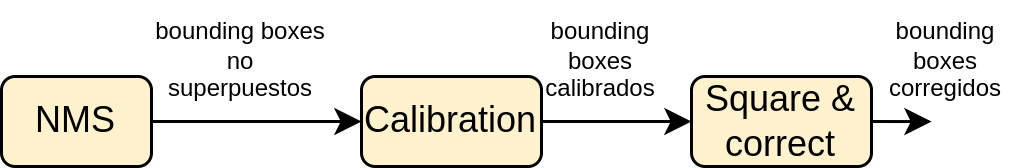
\includegraphics[scale=0.35]{./Figures/mtcnn_postprocess.png}
		\caption{Bloque de postprocesamiento.}
		\label{fig:mtcnn_postprocess}
	\end{figure}
	
	\item \textit{Pre-process}: tiene la función de procesar los datos de entrada para las redes R-Net y O-Net. El primer subbloque genera recortes de la imagen original en función de las coordenadas obtenidas del bloque \textit{post-process}. En el segundo subbloque las imágenes recortadas de entrada son redimensionadas con dimensiones de 24x24 píxeles y 48x48 píxeles para alimentar R-Net y O-Net, respectivamente.`
	\begin{figure}[h]
		\centering
		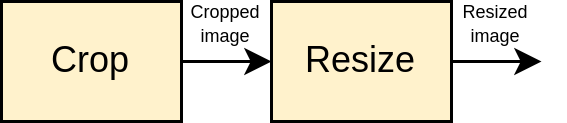
\includegraphics[scale=0.35]{./Figures/mtcnn_preprocess.png}
		\caption{Bloque de preprocesamiento.}
		\label{fig:mtcnn_preprocess}
	\end{figure}

\end{itemize}

P-Net, R-Net y O-Net fueron creados con ayuda de la biblioteca para redes neuronales Keras, que es parte del \textit{core} de TensorFlow, de acuerdo con lo expuesto en \cite{mtcnn_info}. Se generaron 3 modelos de P-Net con diferentes dimensiones para la imagen de entrada, de tal forma que pudieran detectarse rostros a una distancia de entre 1 y 3 metros. Con las arquitecturas definidas de los modelos, el siguiente paso natural en el desarrollo debería haber sido su entrenamiento con uno o varios \textit{datasets}, pero al ser MTCNN tan popular en el ámbito de detección facial se pudieron encontrar archivos de extensión \texttt{.h5} que contenían los \textit{weights} resultantes de un proceso de entrenamiento anterior. En el código \ref{cod:pnets_create} se pueden observar las líneas de código empleadas para crear los modelos de P-Net para TensorFlow.

\begin{lstlisting}[language=Python, label=cod:pnets_create, caption=Código para crear los modelos de P-Net con TensorFlow.]
# Image parameters
w, h, ch = (96, 96, 3) # 96x96 RGB888
scales = [0.3333333, 0.25, 0.125]

# List to store all P-Net models generated for all scales
pnets = []

# Create the models for all the scales
for scale in scales:
  # Get the scaled width and height values
  ws, hs = int(w * scale), int(h * scale)

  # Create the TF model for the current scale and use the pre-trained weigths
  pnet_scale = mtcnn.create_pnet(ws, hs, "mtcnn_esp32s3/models_weights/12net.h5")

  # Append the scaled model to pnets list
  pnets.append(pnet_scale)
\end{lstlisting}

Para que los modelos obtenidos pudieran ser ejecutados en el hardware objetivo de este trabajo tuvieron que ser convertidos a un formato más liviano y eficiente llamado TensorFlow Lite. El conversor de TensorFlow Lite toma un modelo de TensorFlow y genera un modelo de TensorFlow Lite cuya extensión de archivo es \texttt{.flite}. La conversión puede seguir 2 caminos según como sean evaluados los modelos de TensorFlow, en la figura \ref{fig:tf2tflite_workflow} se observa el flujo de trabajo del conversor.

\begin{figure}[h]
	\centering
	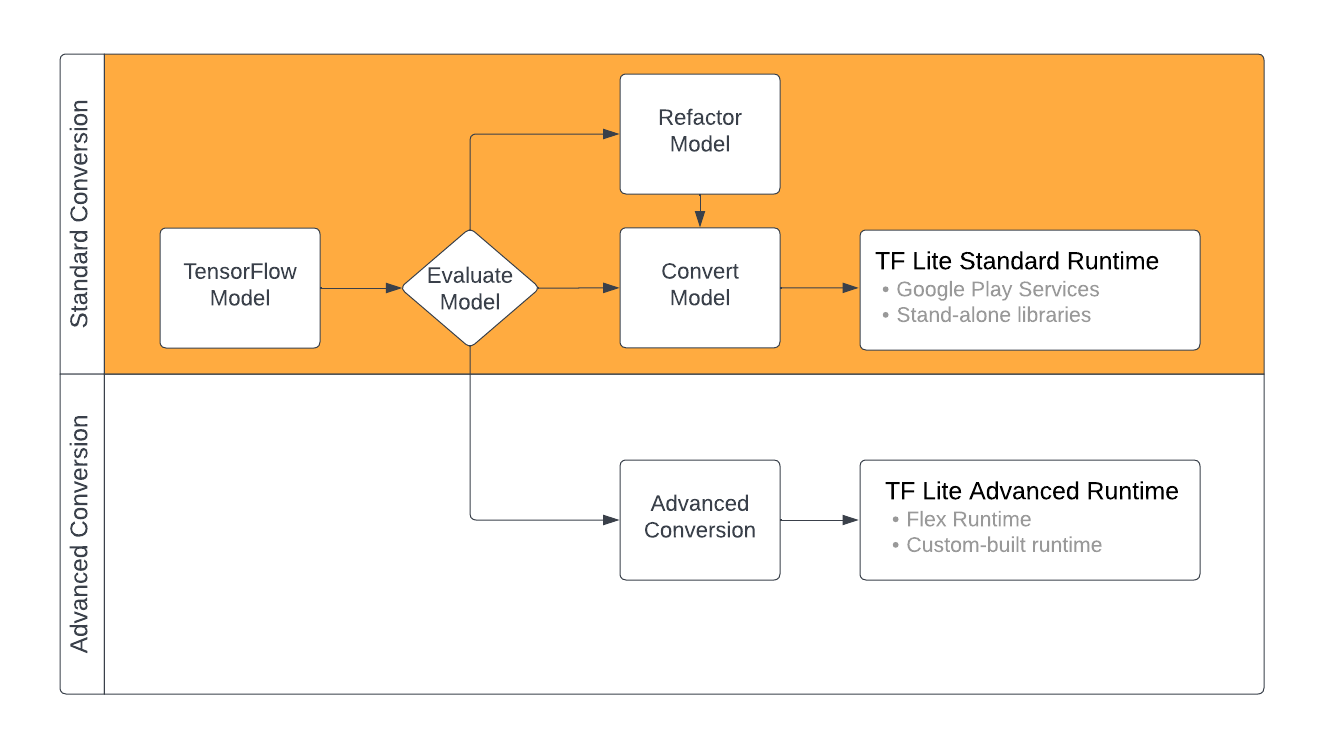
\includegraphics[scale=0.6]{./Figures/tf_convert_workflow_diag.png}
	\caption{Diagrama de flujo de trabajo para la conversion\protect\footnotemark.}
	\label{fig:tf2tflite_workflow}
\end{figure}
\footnotetext{Imagen tomada de: \url{https://www.tensorflow.org/lite/models/convert/}}

Gracias a que todos los operadores utilizados en los modelos de TensorFlow eran compatibles con los operadores de TensorFlow Lite se realizó una conversión estándar, lo que posteriormente facilitó su implementación en el hardware destino.

Durante el proceso de conversión se aplicaron optimizaciones que responden a una necesidad de reducir aún más el tamaño y la latencia de los modelos. Se hizo una optimización por cuantización, que se refiere a la reducción de la precisión de los números usados para representar los parámetros de los modelos, los cuales por defecto son flotantes de 32 bits. Las opciones de cuantización para los modelos se tomaron del diagrama de la figura \ref{fig:tf_quantization_tree}.

\begin{figure}[h]
	\centering
	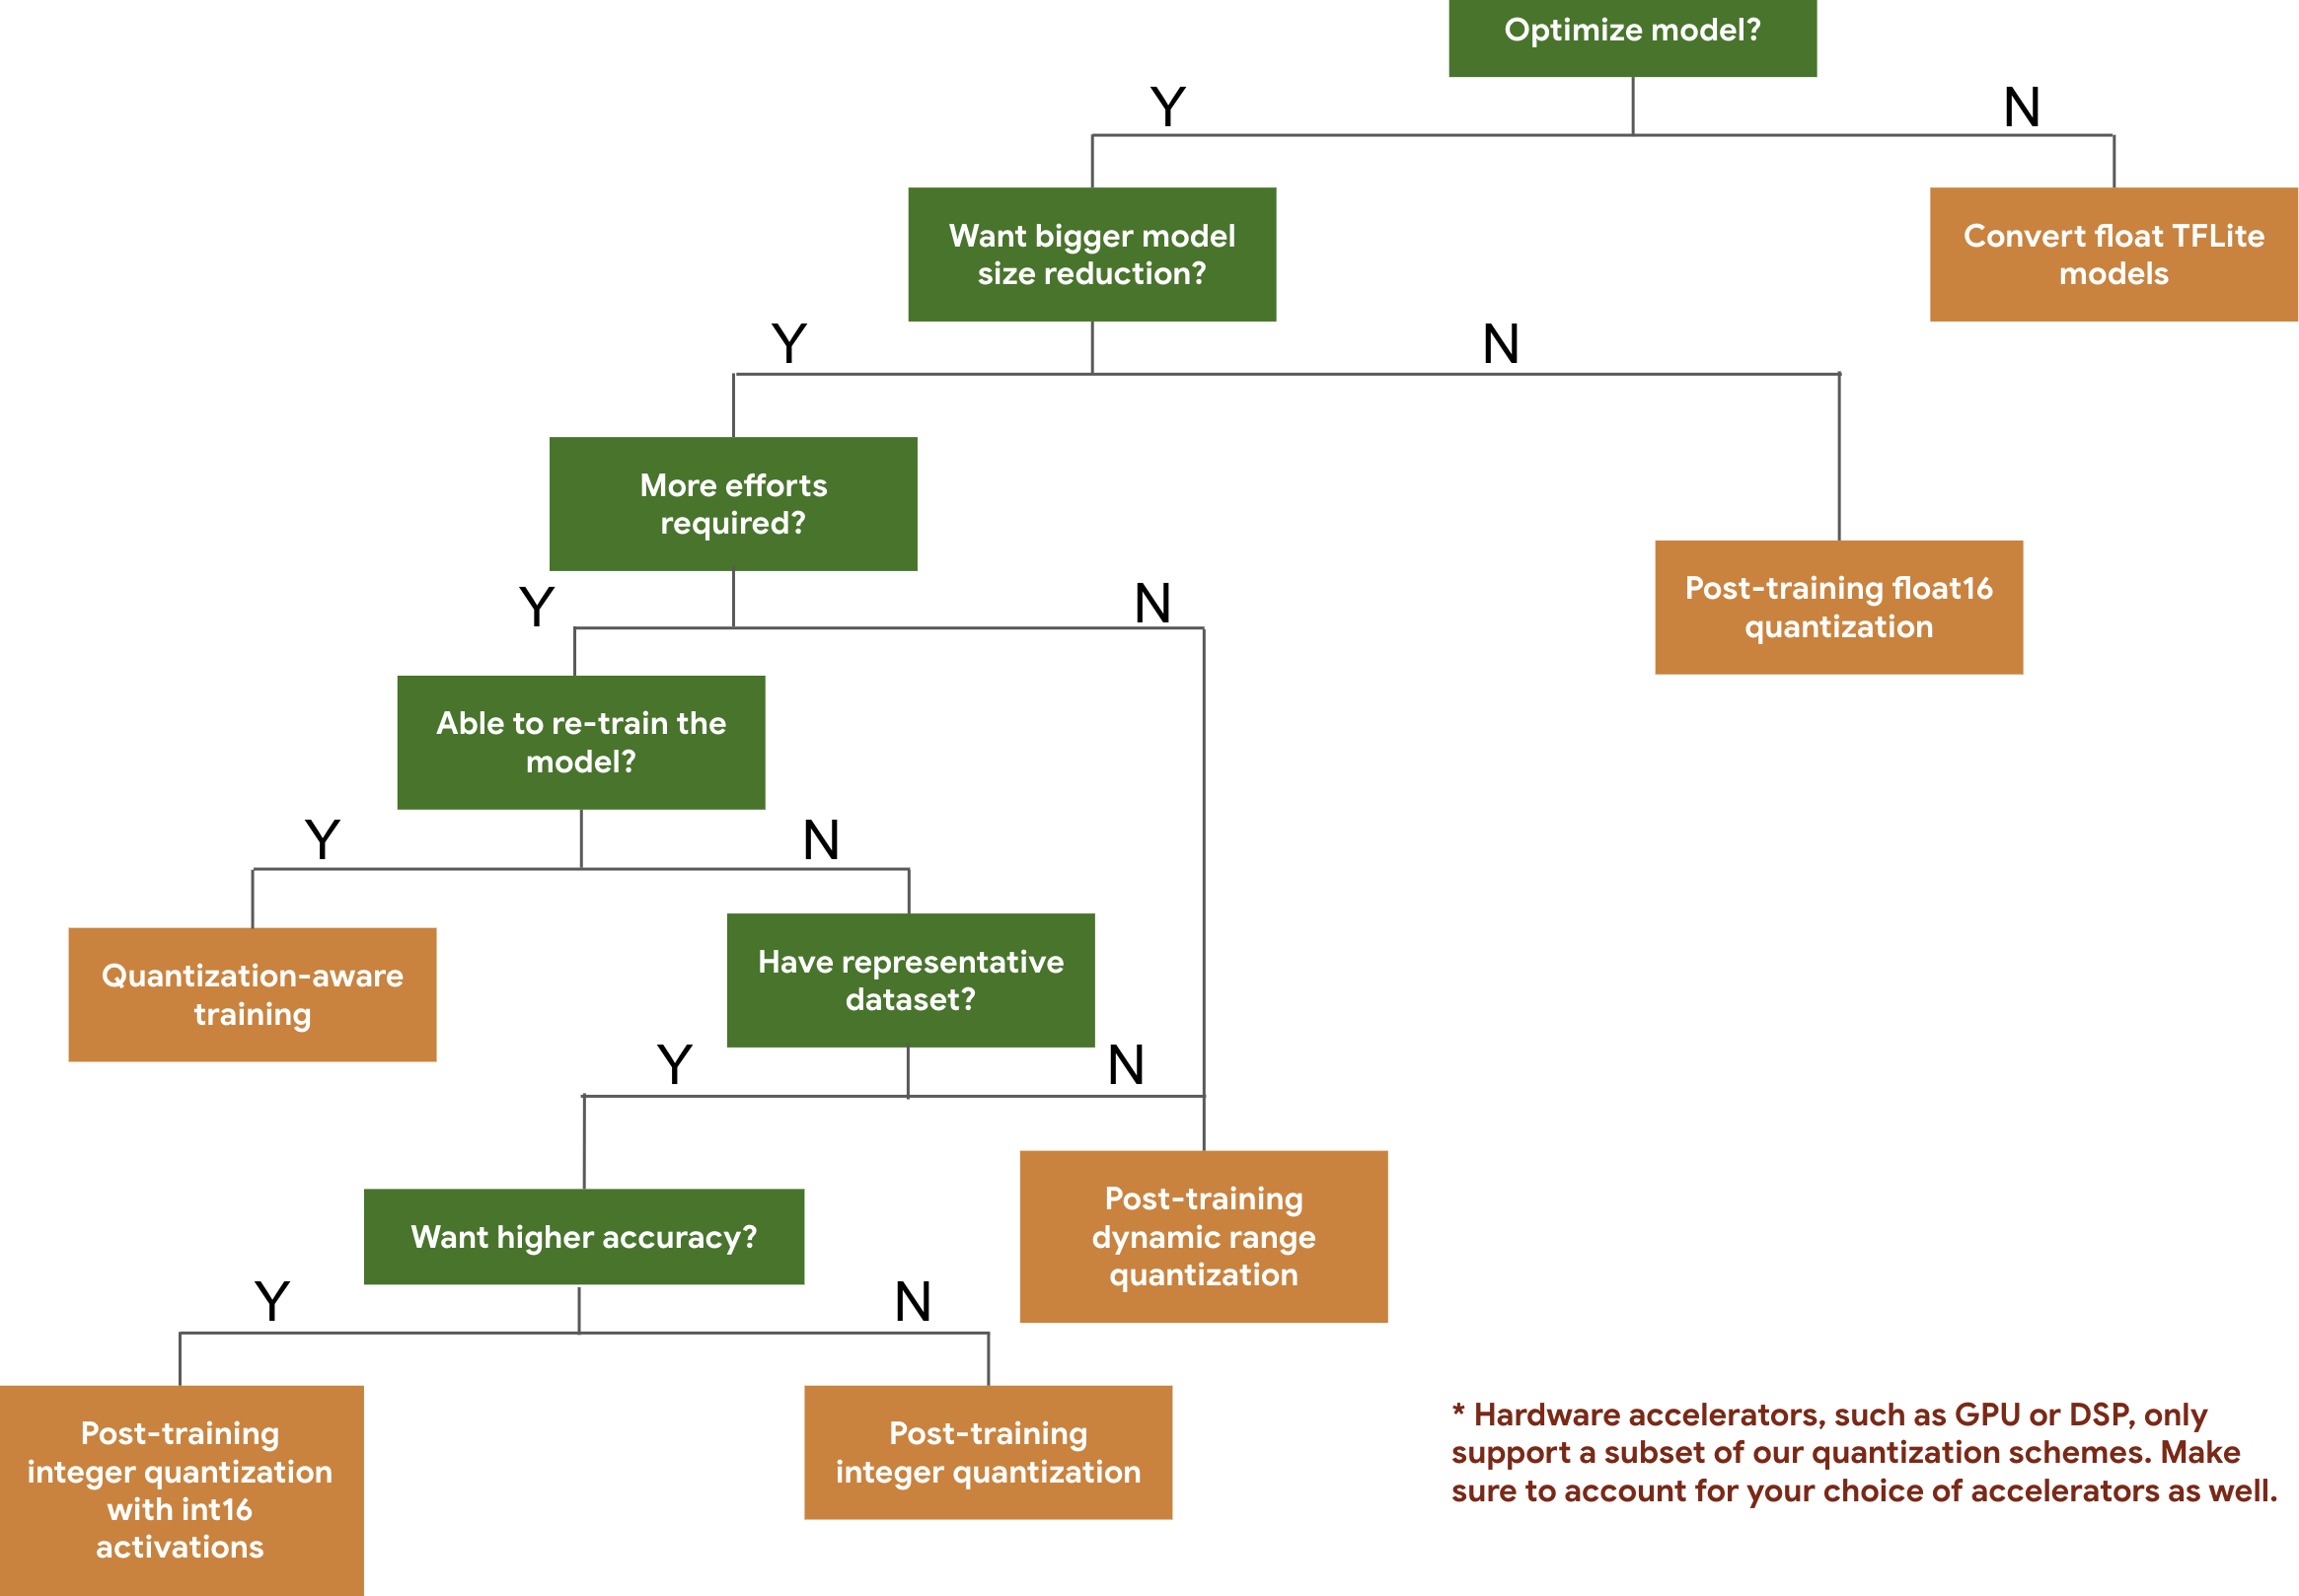
\includegraphics[scale=0.3]{./Figures/tf_quantization_decision_tree.png}
	\caption{Diagrama de árbol de decisiones para el proceso de cuantización\protect\footnotemark.}
	\label{fig:tf_quantization_tree}
\end{figure}
\footnotetext{Imagen tomada de: \url{https://www.tensorflow.org/lite/performance/model_optimization}}

La cuantización utilizada para los modelos fue \textit{full integer quantization}, que reduce los picos de memoria utilizados y asegura la compatibilidad con dispositivos de hardware que no pueden utilizar punto flotante. Para este tipo de cuantización se necesitó crear un \textit{dataset} representativo, compuesto por un pequeño subconjunto (entre 100 a 500 muestras) del \textit{dataset} de entrenamiento. En el código \ref{cod:pnets_tflite} se expone el código empleado para la conversión de los modelos de P-Net en TensorFlow al formato TensorFlow Lite con cuantización a 8 bits.

\begin{lstlisting}[language=Python, label=cod:pnets_tflite, caption=Código para crear los modelos de P-Net con TensorFlow Lite con cuantización de 8 bits.]
# List to store all P-Net int8 quantized models generated for all scales
pnets_quant_int8 = []

# Create the models for all the scales
for pnet_scale in pnets:
  # Function to generate a representative dataset to convert to TF Lite quantized
  def representative_dataset():
    for i, image_file in enumerate(os.listdir("mtcnn_esp32s3/representative_dataset/")):
      image_input = cv2.imread("mtcnn_esp32s3/representative_dataset/" + image_file)
      image_input = np.expand_dims(utils.preprocess_image(image_input, hs, ws, np.float32), axis=0)
      yield [image_input.astype(np.float32)]

  # Convert the TF model to the TF Lite quantized format 
  converter = tf.lite.TFLiteConverter.from_keras_model(pnet_scale)
  converter.optimizations = [tf.lite.Optimize.DEFAULT] # Set the optimization flag
  converter.target_spec.supported_ops = [tf.lite.OpsSet.TFLITE_BUILTINS_INT8] # Enforce integer only quantization
  converter.inference_input_type = tf.int8 # Define the quantization data type
  converter.representative_dataset = representative_dataset # Provide a representative dataset to ensure we quantize correctly.
  pnet_scale_quant_int8 = converter.convert()

  # Append the scaled model to pnets_quant_int8 list
  pnets_quant_int8.append(pnet_scale)
\end{lstlisting}

La tabla \ref{tab:models_comp} muestra los resultados de una prueba de todos los modelos obtenidos con una imagen RGB888, 96x96 píxeles y 3 rostros contenidos.

\begin{table}[h]
	\centering
	\caption[Modelos comparativa]{Tabla comparativa de MTCNN}
	\begin{tabular}{lccc}   
		\toprule
		\textbf{Parámetro} & \textbf{TensorFlow} & \textbf{TensorFlow Lite} & \textbf{TensorFlow Lite int8} \\
		\midrule
		Tamaño (bytes) & - & 2053460 &  556720 \\
		Tiempo de ejecución (ms) & 1.258 & 0.059 & 0.0144 \\
		Rostros & 3 & 3 & 3 \\
		\bottomrule
		\hline
	\end{tabular}
	\label{tab:models_comp}
\end{table}

Todo el código para la obtención de los modelos hasta aquí expuesto, las funciones del \textit{pipeline}, las pruebas realizadas a los modelos y el despliegue de estos en el SoC ESP32-S3, se encuentra disponible en el repositorio del trabajo \cite{mtcnn_repo}.

%----------------------------------------------------------------------------------------
\section{Desarrollo del firmware}
El primer paso para el desarrollo del firmware del dispositivo fue la elección de un conjunto de herramientas de software (SDK, \textit{Software Development Kit}). Estas herramientas permitieron implementar código para utilizar de manera eficiente todos los periféricos disponibles en el ESP32-S3. Para este proyecto el SDK utilizado fue ESP-IDF \cite{idf_repo}, las razones de su elección fueron:
\begin{itemize}
	\item Compatibilidad: casi la totalidad de funciones en el \textit{framework} son compatibles con todos los SoCs de la serie ESP32, salvo por algunas que solo son útiles para algunos periféricos que no se encuentran disponibles en todos los SoCs.
	\item Herramientas: además del código para manejar los periféricos de los SoCs ESP32, posee herramientas que son muy útiles para crear particiones, grabar código en memoria, aprovisionamiento de credenciales Wi-Fi, entre otras.
	\item Soporte: existen foros y sitios web especializados en el soporte de fimware y hardware para los SoCs de Espressif.
	\item Documentación: ESP-IDF está muy bien documentado y se dispone de muchos ejemplos que implementan las funciones de su \textit{framework}
\end{itemize}

Con el conjunto de herramientas definido, otro aspecto de importancia fue la elección de un entorno de desarrollo para optimizar la escritura y depuración del código. El entorno de desarrollo integrado (IDE, \textit{Integrated Development Environment}) escogido fue Eclipse IDE C/C++, los aspectos más importantes para su elección fueron:
\begin{itemize}
	\item Herramientas: posee muchas herramientas interesantes como integración con Git, Valgrind y análisis de código, entre otros.
	\item Complementos: se pueden instalar diferentes tipos de \textit{plugins} para aumentar la utilidad del IDE, para este trabajo se instaló el \textit{plugin} ESP-IDF.
\end{itemize}

Otra herramienta importante para el proceso de desarrollo del firmware fue la utilización de software para control de versiones, que permite realizar un seguimiento de los cambios realizados en el código a lo largo del tiempo. Git fue elegido como software de control de versiones, mientras que GitHub como plataforma para alojar el repositorio de Git. Las razones para la elección de ambos son:
\begin{itemize}
	\item Reutilización de código: se puede reutilizar código en forma de submódulos y tener los componentes de firmware descentralizados de la aplicación principal.
	\item Soporte: el soporte para el uso de Git y GitHub es extenso, se encuentra fácilmente en sus páginas web oficiales y en foros especializados.
\end{itemize}

Con todas las herramientas de software correctamente seleccionadas, el siguiente paso fue el diseño de la arquitectura del firmware. El firmware desarrollado siguió una arquitectura en capas, donde las capas de niveles más bajos tienen una mayor interacción con el hardware, mientras que las de niveles más altos con la aplicación del usuario. En la figura \ref{fig:fw_layers} se presenta el diagrama en capas del firmware.

\begin{figure}[h]
	\centering
	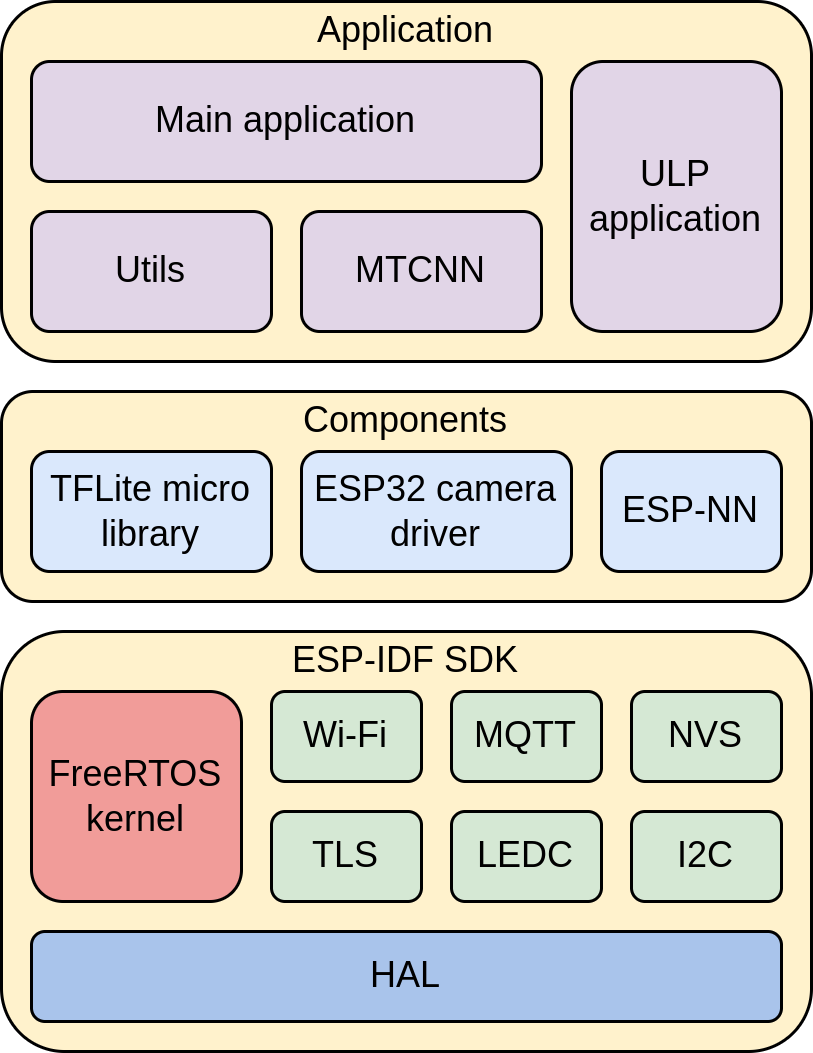
\includegraphics[scale=0.2]{./Figures/fw_layers.png}
	\caption{Diagrama de capas del firmware.}
	\label{fig:fw_layers}
\end{figure}

Las capas expuestas en el diagrama de la figura \ref{fig:fw_layers} son:
\begin{itemize}
	\item ESP-IDF SDK: esta capa se encuentra compuesta por el \textit{framework} ESP-IDF, que contiene todo el código necesario para controlar los periféricos del ESP32-S3.
	\item \textit{Components}: esta capa está conformada por submódulos de código de Git que se encargan de controlar los componentes adicionales de hardware y las bibliotecas de código de terceros. En el repositorio del trabajo \cite{mtcnn_repo} está representada por la carpeta \texttt{components/}.
	\begin{itemize}
		\item TFLite micro library: biblioteca de código de TensorFlow Lite para microcontroladores \cite{tflm_repo}.
		\item ESP32 camera driver: biblioteca de código para controlar diversos modelos cámaras con los SoCs ESP32 \cite{esp32cam_repo}.
		\item ESP-NN: biblioteca de código que implementa funciones que se utilizan para ejecutar algoritmos de ML y DL en los SoCs ESP32 \cite{espnn_repo}.
	\end{itemize}
	\item \textit{Application}: esta capa contiene el código de aplicación del dispositivo. La carpeta \texttt{main/} del repositorio del trabajo \cite{mtcnn_repo} contiene todos sus archivos.
	\begin{itemize}
		\item \textit{Main application}: código de la aplicación que corre en los procesadores principales, donde se ejecutan los procesos de detección facial y conexión con los servicios en la nube. El código se encuentra en el archivo \texttt{main/main.cc}
		\item \textit{ULP application}: código de la aplicación que se ejecuta en el coprocesador ULP, se emplea principalmente para ejecutar la aplicación principal con el menor gasto energético posible. El código de este bloque se encuentra en el archivo \texttt{main/ulp/main.c}
		\item MTCNN: biblioteca de código que implementa las funciones del \texttt{pipeline} de MTCNN. Los archivos que contiene su código son \texttt{main/mtcnn.cc} y \texttt{main/mtcnn.h}
		\item \textit{Image utils}: código que implementa funciones para el procesamiento de imágenes. Está compuesto por los archivos \texttt{main/image\_utils.c} e \texttt{main/image\_utils.h}
	\end{itemize}
\end{itemize}

El firmware desarrollado cumple principalmente con las siguientes tareas: detección facial con TensorFlow Lite Micro, comunicación con los servicios en la nube y gestión del consumo energético.

\subsection{Detección facial con TensorFlow Lite Micro}
El objetivo de esta tarea es obtener imágenes con la cámara del sistema para procesarlas con los modelos de MTCNN para TensorFlow Lite para microcontroladores y determinar la cantidad de rostros humanos existentes en cada imagen. El diagrama de flujo de la figura \ref{fig:fw_detect_flow} detalla el proceso de esta tarea.

\begin{figure}[h]
	\centering
	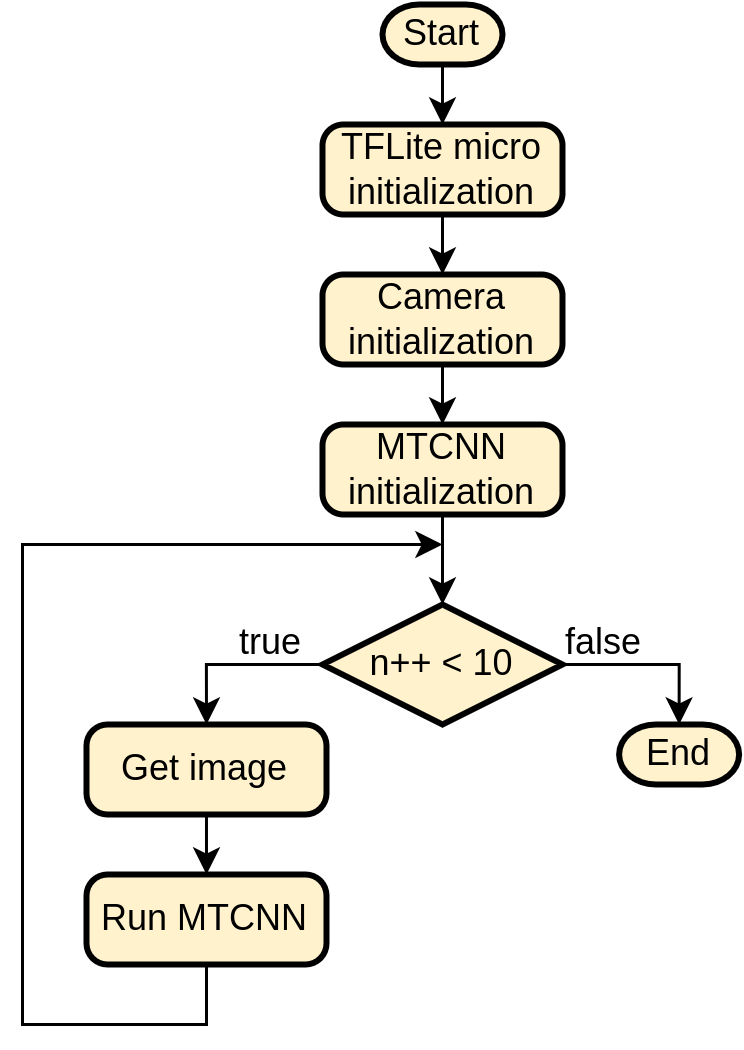
\includegraphics[scale=0.22]{./Figures/fw_detection_flow.png}
	\caption{Diagrama de flujo de la tarea de detección facial.}
	\label{fig:fw_detect_flow}
\end{figure}

El proceso de inicialización de TFLite micro requiere de varios pasos que deben ser seguidos en orden para poder ejecutar los modelos de MTCNN correctamente. En el código \ref{cod:tflm_init} se presentan las líneas de código necesarias para la inicialización de O-Net con TFLite micro.

\begin{lstlisting}[label=cod:tflm_init,caption=Código para inicializar O-Net con TFLite micro.]
/* Map the model into a usable data structure */
const tflite::Model *onet_model = tflite::GetModel(onet_model_data);

/* Reserve memory for the tensors */
uint8_t *tensor_arena = (uint8_t *)heap_caps_malloc(TENSOR_ARENA_SIZE, MALLOC_CAP_SPIRAM | MALLOC_CAP_8BIT);

/* Pull in only the operation implementations needed */
static tflite::MicroMutableOpResolver<10> micro_op_resolver;
micro_op_resolver.AddAveragePool2D();
micro_op_resolver.AddConv2D();
micro_op_resolver.AddPrelu();
micro_op_resolver.AddMaxPool2D();
micro_op_resolver.AddTranspose();
micro_op_resolver.AddFullyConnected();
micro_op_resolver.AddDequantize();
micro_op_resolver.AddDepthwiseConv2D();
micro_op_resolver.AddReshape();
micro_op_resolver.AddSoftmax();

/* Build an interpreter to run the model with */
static tflite::MicroInterpreter static_onet_interpreter(onet_model, micro_op_resolver, tensor_arena, TENSOR_ARENA_SIZE);
onet_interpreter = &static_onet_interpreter;

/* Allocate memory from the tensor_arena for the model's tensors */
onet_interpreter->AllocateTensors();
\end{lstlisting}

Los modelos de P-Net y R-Net se inicializan de la misma forma que O-Net y una cosa a notar es la declaración de los operadores estrictamente necesarios para ejecutar estos modelos en las líneas 9 a 18. Otra aproximación más sencilla era utilizar \texttt{OpsResolver} para utilizar todos los operadores, pero esto hubiera supuesto una penalización en la cantidad de memoria RAM utilizada. En la figura \ref{fig:fw_tflite_ops} se puede observar una captura de pantalla de una página web generada con la herramienta de visualización de modelos de TensorFlow Lite que se encuentra en el repositorio oficial de TensorFLow Lite para microcontroladores\cite{tflm_repo}, donde se muestran los operadores empleados por O-Net.

\begin{figure}[h]
	\centering
	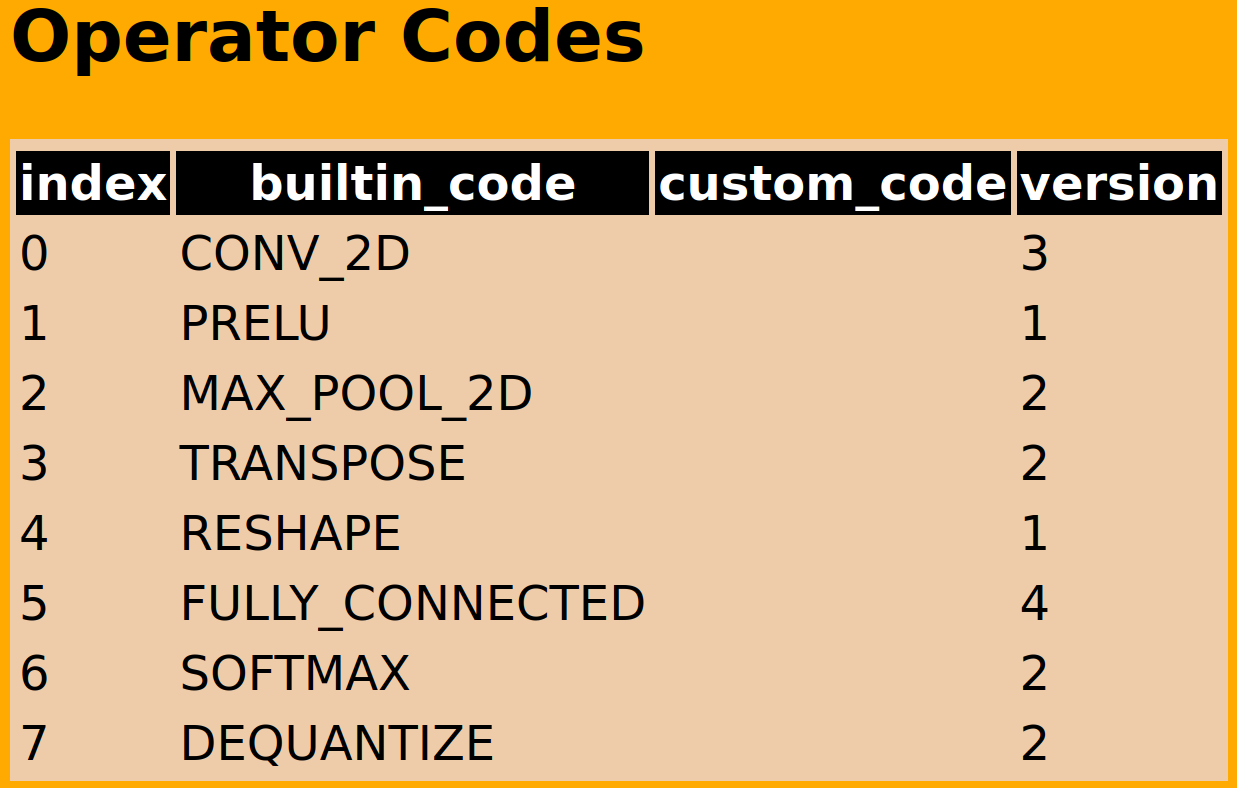
\includegraphics[scale=0.15]{./Figures/fw_tflite_ops.png}
	\caption{Captura de pantalla del detalle del modelo O-Net para TensorFlow Lite.}
	\label{fig:fw_tflite_ops}
\end{figure}

Otro aspecto a destacar es la utilización de la memoria RAM pseudoestática (PSRAM, \textit{Pseudo static} RAM) para almacenar los tensores empleados durante la ejecución de los modelos de MTCNN. En la línea 5 del fragmento de código \ref{cod:tflm_init} se puede observar como se reserva memoria en la PSRAM de un tamaño determinado de manera experimental y denominado \texttt{TENSOR\_ARENA\_SIZE}.

Los métodos de MTCNN para inicializarlo y ejecutar sus modelos se encuentran en los archivos \texttt{main/mtcnn.h} y \texttt{mtcnn.cc} del repositorio \cite{mtcnn_repo}. En el código \ref{cod:mtcnn_struct} se pueden observar las estructuras de datos usados por los métodos de MTCNN.

\begin{lstlisting}[label=cod:mtcnn_struct,caption=Estructura de datos de MTCNN.]
typedef struct {
  tflite::MicroInterpreter *interpreter;
  candidate_windows_t candidate_windows;
  bboxes_t bboxes;
} model_data_t;

typedef struct {
  model_data_t pnet[3];
  model_data_t rnet;
  model_data_t onet;
} mtcnn_t;
\end{lstlisting}

Como el tipo de dato \texttt{mtcnn\_t} contiene todos los datos de entrada y salida de los modelos de MTCNN, fue utilizado como parámetro de todas las funciones encargadas de ejecutar los modelos. La función que ejecuta O-Net es \texttt{mtcnn\_run\_onet} y en el código \ref{cod:run_onet} se puede observar su implementación.

\begin{lstlisting}[label=cod:run_onet,caption=Función mtcnn\_run\_onet.]
void mtcnn_run_onet(mtcnn_t *mtcnn, uint8_t *img, uint16_t img_w, uint16_t img_h) {
  /* Pre-process R-Net ouputs */
  
  /* Feed the model and run it */
  TfLiteTensor *input = mtcnn->interpreter->input(0);
    
  for(int i = 0; i < ONET_SIZE * ONET_SIZE * 3; i++) {
    input->data.int8[i] = ((uint8_t *) onet_image)[i] ^ 0x80;
  }
  
  mtcnn->interpreter->Invoke();
  
  /* Store the scores and offsets output */
  TfLiteTensor *scores = interpreter->output(0);
  
  for(uint8_t j = 0; j < 2; j++) {
    probs_buf[j + (i * 2)] = probs->data.f[j];
  }

  TfLiteTensor *offsets = interpreter->output(1);

  for(uint8_t j = 0; j < 4; j++) {
    offsets_buf[j + (i * 2)] = offsets->data.f[j];
  }
  
  /* Add the candidate windows to the candidate windows array */
  add_candidate_windows();
  
  /* Post-process O-Net ouputs */
}
\end{lstlisting}

\subsection{Comunicación con los servicios en la nube}
Esta tarea fue diseñada para establecer conectividad con los servicios en la nube, más precisamente con el servicio IoT Core de AWS, para transmitir y recibir datos mediante el protocolo MQTT. El diagrama de flujo de la figura \ref{fig:fw_comm_flow} muestra el proceso que sigue esta tarea.

\begin{figure}[h]
	\centering
	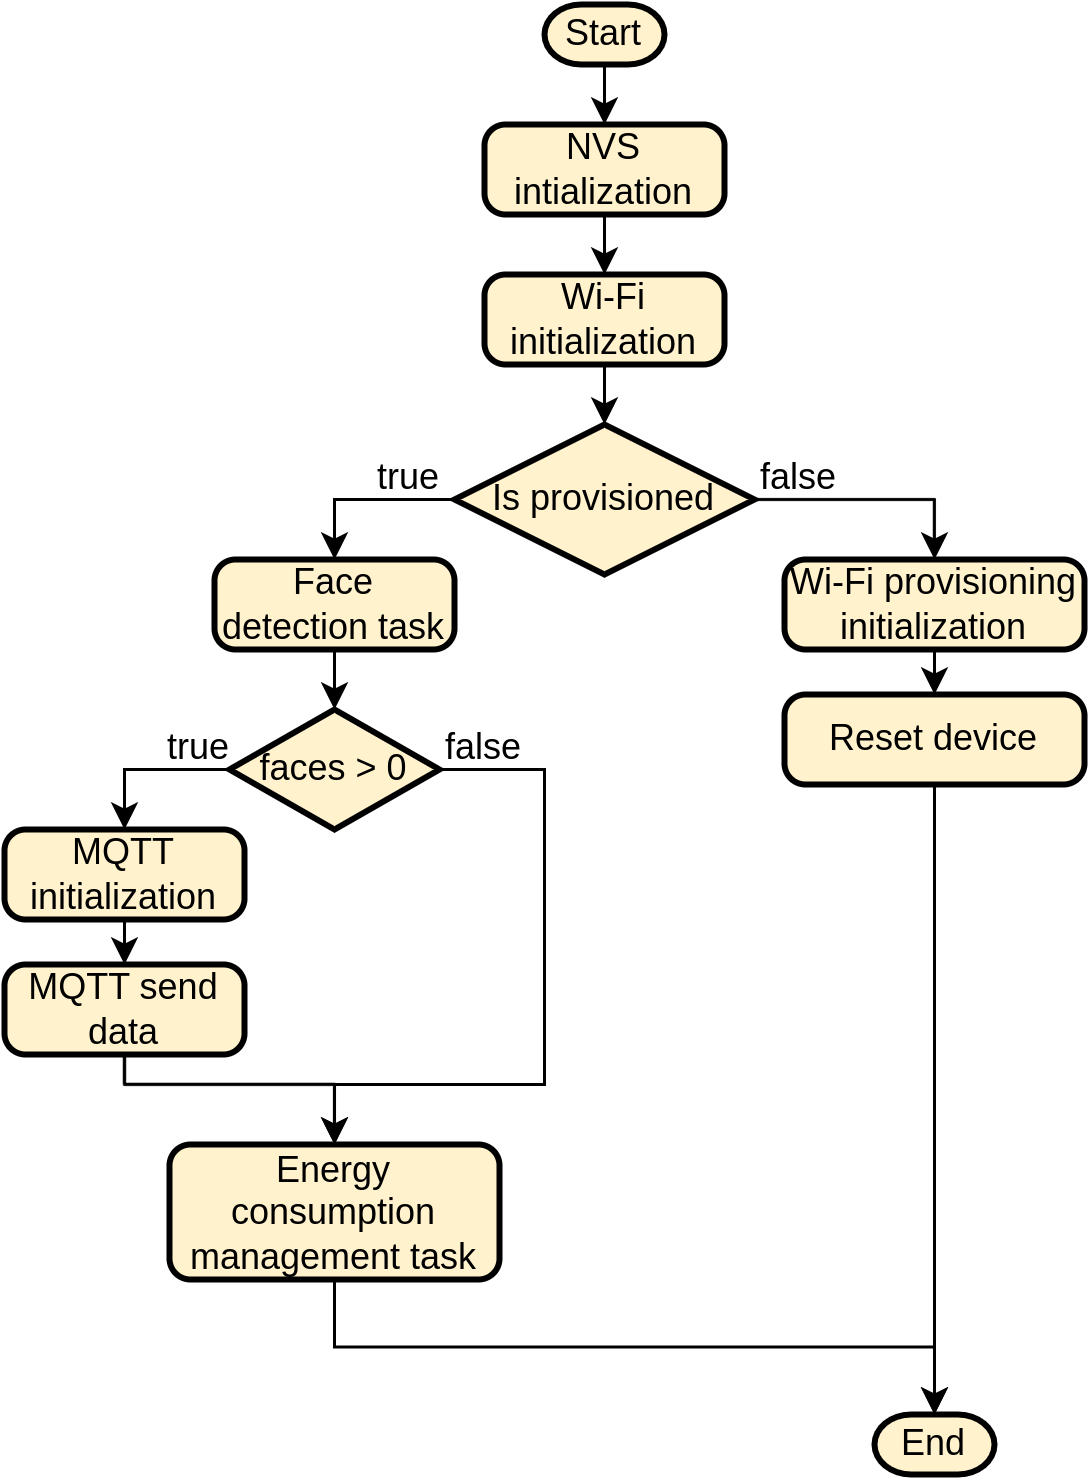
\includegraphics[scale=0.22]{./Figures/fw_comm_flow.png}
	\caption{Diagrama de flujo de la tarea de comunicación con los servicios en la nube.}
	\label{fig:fw_comm_flow}
\end{figure}

El diagrama de la figura \ref{fig:fw_comm_flow} empieza con la inicialización de la memoria NVS y el periférico Wi-Fi en modo punto de acceso y estación a la vez, para después determinar si el dispositivo debe ejecutar el proceso de aprovisionamiento de credenciales Wi-Fi o si debe ejecutar la tarea de detección facial y transmitir los datos generados. Los mensajes se publican en el tópico \texttt{faceCounter} y contienen los datos de identificación del dispositivo, cantidad de rostros detectados, estado de la batería y temperatura del dispositivo. El formato de los mensajes a publicar se muestra en el código \ref{cod:message_json}.

\begin{lstlisting}[label=cod:message_json,caption=Formato de los mensajes a publicar.]
{
   "id":"abddeab5-3428-4129-bbaf-dab22e15d978",
   "payload":{
      "faces":3,
      "battery":89,
      "temp":24
   }
}
\end{lstlisting}

Cuando uno más rostros son detectados por la tarea de detección facial, esta información se transmite por MQTT. AWS IoT Core dispone de un \textit{broker} MQTT que implementa TLS \cite{tls_doc} para brindar seguridad en el intercambio de mensajes, por tanto, la autenticación y cifrado de datos necesita de certificados y llaves para llevarse a cabo. La llave privada y el certificado del dispositivo son generados en la plataforma AWS IoT Core y deben quedar grabadas en la memoria del ESP32-S3 para que puedan ser utilizadas en el código. La forma más simple de usar la llave y el certificado es añadirlas al binario de la aplicación durante el proceso de compilación, en la figura \ref{fig:fw_parttab1} se observa un diagrama representativo de la distribución de la memoria del ESP32-S3, donde los valores encima de los bloques son las posiciones de memoria donde se encuentran las particiones y los valores que se encuentran por debajo son la cantidad de memoria empleada.

\begin{figure}[h]
	\centering
	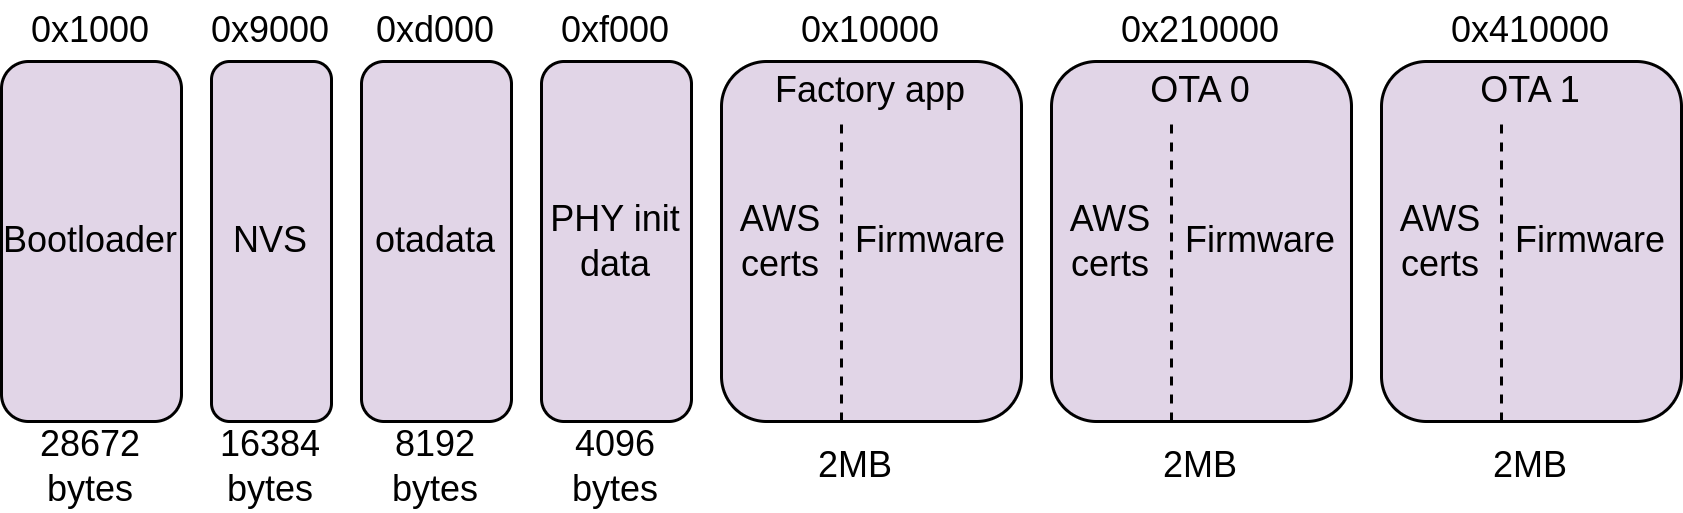
\includegraphics[scale=0.22]{./Figures/fw_parttab1.png}
	\caption{Diagrama representativo de la memoria del ESP32-S3.}
	\label{fig:fw_parttab1}
\end{figure}

En el diagrama de la figura \ref{fig:fw_parttab1} se puede observar un problema no menor con respecto a al proceso de actualizaciones OTA, que las actualizaciones sobreescribirán tanto el \textit{firmware} como el certificado y llave privada del dispositivo. Esto no sería problemático para un solo dispositivo, pero si existieran más dispositivos establecerían conexión con AWS IoT Core con el mismo certificado y llave privada, lo que supondría una grave falla de seguridad de la información. Para corregir esta falla de seguridad se optó por generar llaves y certificados únicos para cada dispositivo, y grabarlos en la memoria NVS en un \textit{namespace} llamado "certs", de esta forma el proceso de actualización OTA solo sobreescribirá el \textit{firmware} más no el certificado ni la llave. En la figura \ref{fig:fw_parttab2} se muestra el diagrama representativo de la memoria del ESP32-S3 utilizado en este trabajo.

\begin{figure}[h]
	\centering
	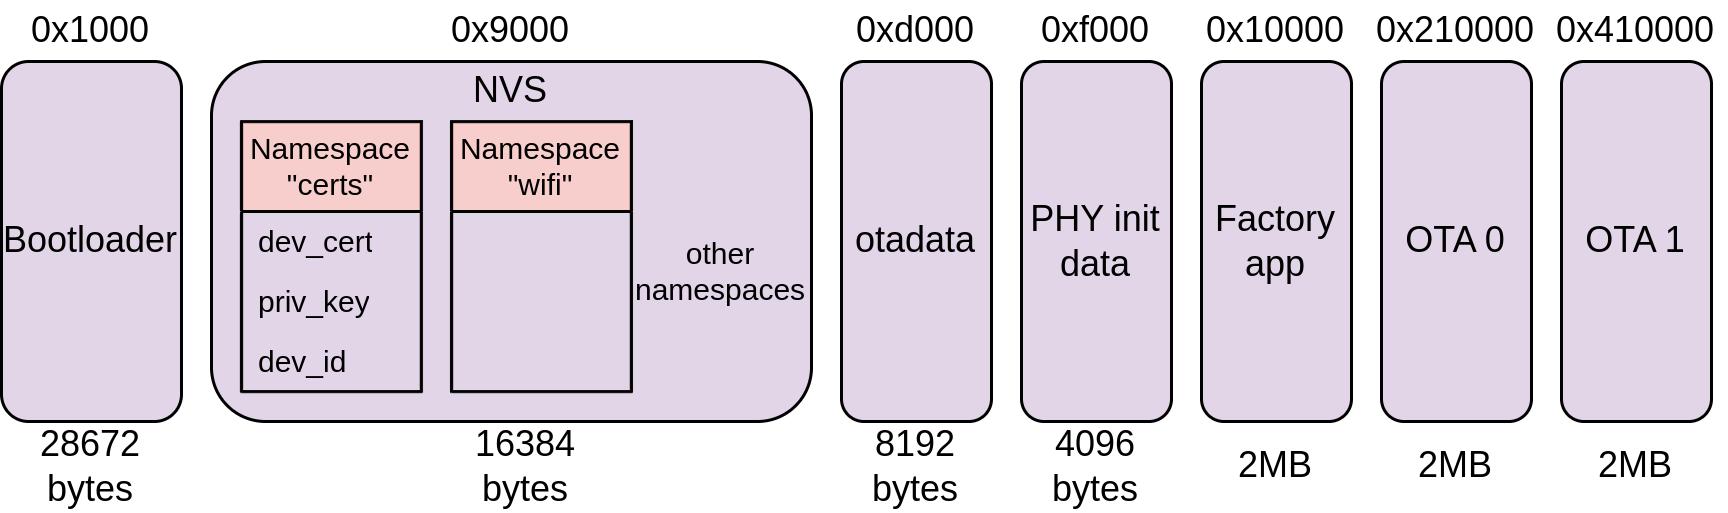
\includegraphics[scale=0.22]{./Figures/fw_parttab2.png}
	\caption{Diagrama representativo de la memoria del ESP32-S3.}
	\label{fig:fw_parttab2}
\end{figure}

La inicialización de MQTT en el código utiliza una estructura de datos donde algunos campos deben ser asignados al certificado del dispositivo y la llave privada en formato de cadena de caracteres. En los códigos \ref{cod:nvs_string} y \ref{cod:mqtt_client} se exhiben la función para obtener una cadena de caracteres de la NVS y la inicialización de MQTT en modo cliente, respectivamente.

\begin{lstlisting}[label=cod:nvs_string,caption=Función para cargar una cadena de caracteres de la NVS.]
esp_err_t load_string_from_nvs(const char * namespace_name, const char *key, char **value) {
  esp_err_t ret = ESP_OK;
  nvs_handle_t nvs_handle;
  size_t value_size;

  /* Open the name space to read and write */
  ret = nvs_open(namespace_name, NVS_READONLY, &nvs_handle);

  if (ret != ESP_OK) {
	ESP_LOGE(TAG, "Error opening namespace %s", namespace_name);
	return ret;
  }

  /* Get value size */
  ret = nvs_get_str(nvs_handle, key, NULL, &value_size);

  if (ret != ESP_OK){
	ESP_LOGE(TAG, "Failed to get size of key: %s", key);
    return ret;
  }

  /* Allocate memory and get value */
  *value = (char *)malloc(value_size);
  ret = nvs_get_str(nvs_handle, key, * value, &value_size);

  if (ret != ESP_OK){
	 ESP_LOGE(TAG, "Failed to load key: %s", key);
     return ret;
  }

  /* Close NVS and return */
  nvs_close(nvs_handle);
  return ret;
}
\end{lstlisting}

\begin{lstlisting}[label=cod:mqtt_client,caption=Código para inicializar MQTT en modo cliente.]
/* CA certificate is embedded in the binary application */
extern const char amazon_root_ca1_pem_start[] asm("_binary_amazon_root_ca1_pem_start");

/* Get device certificate and private key from NVS */
char *device_cert = NULL;
char *priv_key = NULL;

load_string_from_nvs("certs", "dev_cert", &dev_cert);
load_string_from_nvs("certs", "priv_key", &priv_key);

/* Fill MQTT client configuration */
const esp_mqtt_client_config_t mqtt_config = {
  .broker = {
    .address = {
      .uri = BROKER_URL, /* Broker address in port 8883 */
    },
	.verification = {
      .certificate = (const char *)amazon_root_ca1_pem_start,
    },
  },
  .credentials = {
    .authentication = {
      .certificate = (const char *)dev_cert,
      .key = (const char *)priv_key
    },
  },
};

/* Initialize MQTT client */
mqtt_client = esp_mqtt_client_init(&mqtt_config);
\end{lstlisting}

\subsection{Gestión del consumo energético}
Esta tarea reduce el consumo promedio de corriente del dispositivo para lograr que pueda ser operado por 2 baterías AA de litio durante un tiempo prolongado. Hace uso del coprocesador ULP del ESP32-S3 para correr un programa que monitorea el estado del sensor de movimiento en un determinado intervalo de tiempo, para determinar si el procesador principal debe ser despertado para ejecutar las tareas de detección facial y comunicación con los servicios en la nube. Para utilizar el coprocesador ULP se debe configurar e inicializar como se muestra en el código \ref{cod:ulp_init}.

\begin{lstlisting}[label=cod:ulp_init,caption=Código para inicializar el coprocesador ULP.]
/* Initialize selected GPIO as RTC IO, enable input, disable pullup and pulldown */
rtc_gpio_init(PIR_GPIO);
rtc_gpio_set_direction(PIR_GPIO, RTC_GPIO_MODE_INPUT_ONLY);
rtc_gpio_pulldown_dis(PIR_GPIO);
rtc_gpio_pullup_dis(PIR_GPIO);
rtc_gpio_hold_en(PIR_GPIO);

/* Declare the embedded ULP app */
extern const uint8_t ulp_main_bin_start[] asm("_binary_ulp_main_bin_start");
extern const uint8_t ulp_main_bin_end[]   asm("_binary_ulp_main_bin_end");

/* Load the ULP application */
ulp_riscv_load_binary(ulp_main_bin_start, (ulp_main_bin_end - ulp_main_bin_start));

/* Configure the timer to wake up de ULP co-processor */
ulp_set_wakeup_period(0, 300000); /* 300 ms */

/* Start the ULP program */
ulp_riscv_config_and_run(&cfg);

/* Enable the wakeup source */
esp_sleep_enable_ulp_wakeup();

/* Start deep sleep */
esp_deep_sleep_start();
\end{lstlisting}

El funcionamiento del coprocesador ULP sigue una secuencia que puede ser explicada con ayuda del diagrama de la figura \ref{fig:ulp_sequence}.

\begin{figure}[h]
	\centering
	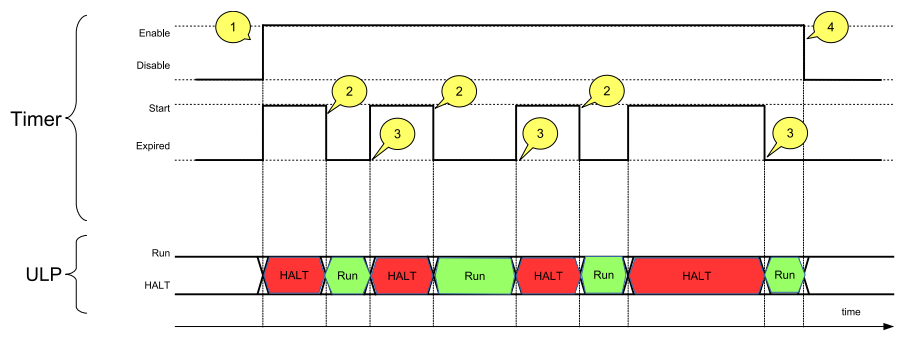
\includegraphics[scale=0.43]{./Figures/ulp_sequence.png}
	\caption{Diagrama de la secuencia de operación del coprocesador ULP del ESP32-S3\protect\footnotemark.}
	\label{fig:ulp_sequence}
\end{figure}
\footnotetext{Imagen tomada de: \url{https://www.espressif.com/sites/default/files/documentation/esp32-s3_technical_reference_manual_en.pdf}}

\begin{enumerate}
	\item Se habilita el \textit{timer} y empieza su conteo.
	\item El \textit{timer} expira y despierta al coprocesador ULP. El coprocesador ULP empieza la ejecución de su programa. 
	\item El coprocesador ULP se pone en estado \textit{halt}, es decir, detiene su funcionamiento, y el \textit{timer} comienza su conteo de nuevo.
	\item Se deshabilita el \textit{timer} mediante el programa del coprocesador ULP o el programa del procesador principal.
\end{enumerate}

El sensor de movimiento está basado en un diseño de Texas Instruments \cite{pir_ti} que utiliza el TLV8544 para lograr una aplicación de ultra bajo consumo de detección de movimiento humano. El sensor genera un nivel lógico alto en su salida cuando detecta movimiento en un rango de 4 metros y consume aproximadamente 2 \textmu A. Pero al trabajar con corrientes de polarización tan pequeñas, la salida del sensor tiende a generar señales de muy corta duración o falsos positivos como se muestra en la figura \ref{fig:ulp_pir_noise}

\begin{figure}[h]
	\centering
	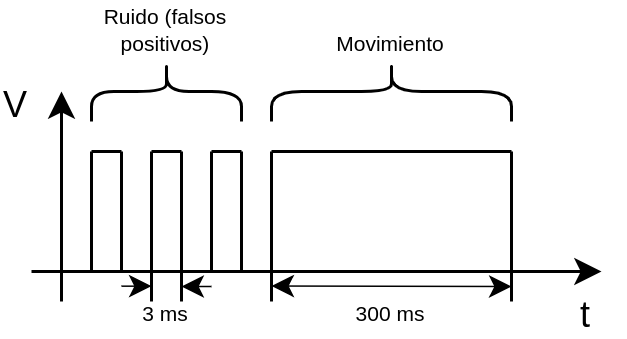
\includegraphics[scale=0.40]{./Figures/ulp_pir_noise.png}
	\caption{Diagrama de la secuencia de operación del coprocesador ULP del ESP32-S3.}
	\label{fig:ulp_pir_noise}
\end{figure}

Para evitar que el procesador principal se active por la aparición de falsos positivos generados por el sensor de movimiento, se diseñó una máquina de estados que corre en el coprocesador ULP. Esta máquina de estados tiene la función de filtrar todas las señales de nivel lógico alto con una duración menor a 300 ms y está basada en el diagrama de la figura \ref{fig:ulp_fsm}.

\begin{figure}[h]
	\centering
	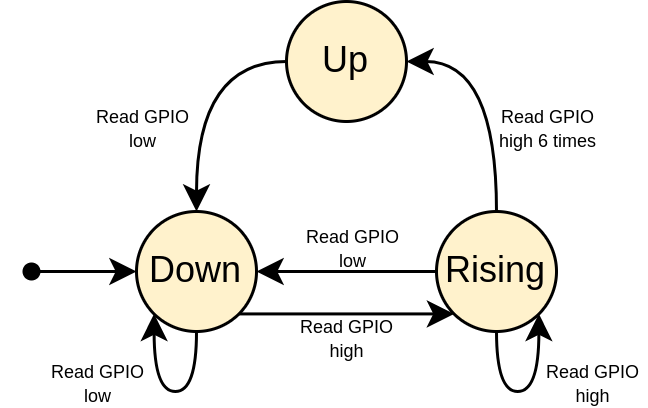
\includegraphics[scale=0.40]{./Figures/ulp_fsm.png}
	\caption{Máquina de estados para filtar falsos positivos del sensor de movimiento.}
	\label{fig:ulp_fsm}
\end{figure}

Con todas las técnicas de bajo consumo aplicadas hasta ahora, el funcionamiento del dispositivo se puede describir como la transición entre todos sus modos de consumo, tal como se muestra en la figura \ref{fig:ulp_modes}.

\begin{figure}[h]
	\centering
	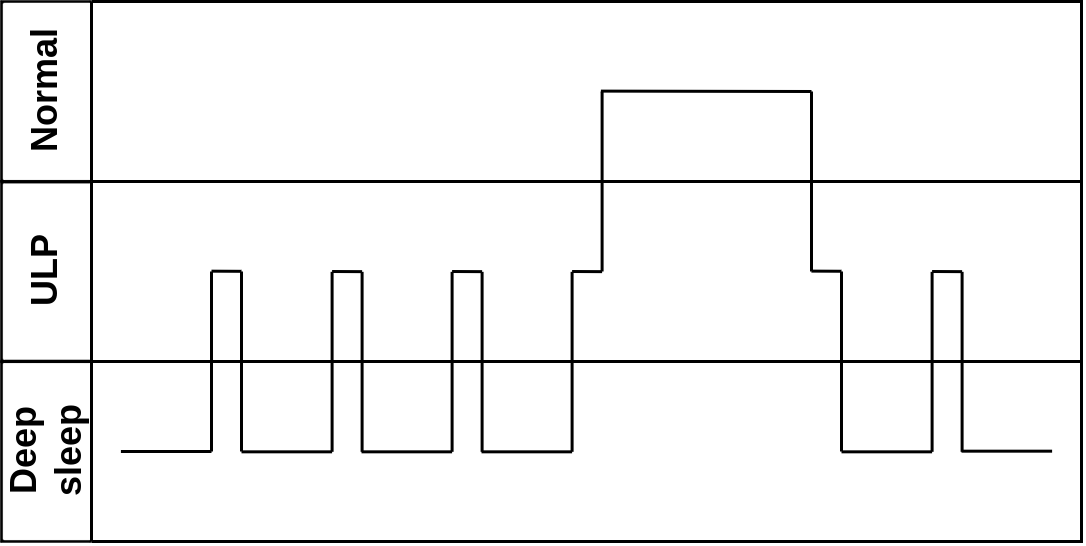
\includegraphics[scale=0.3]{./Figures/ulp_modes.png}
	\caption{Diagrama de transición de modos de consumo del dispositivo.}
	\label{fig:ulp_modes}
\end{figure}

La mayor parte del tiempo de funcionamiento el dispositivo se encontrará entre los modos \textit{deep sleep} y ULP, hasta que el sensor de movimiento genere una señal de suficiente duración y se cambie al estado normal, donde se ejecutan las tareas de detección facial y comunicación con los servicios en la nube. En la tabla \ref{tab:ulp_table} se muestran los valores de corriente utilizados por el dispositivo en cada uno de los estados de funcionamiento.

\begin{table}[h]
	\centering
	\caption[Consumo de corriente del dispositivo]{Consumo de corriente aproximado de todos los modos del dispositivo}
	\begin{tabular}{lc}   
		\toprule
		\textbf{Estado} & \textbf{Consumo (mA)}  \\
		\midrule
		Normal & 400 \\
		ULP & 0.2 \\
		\textit{Deep sleep} & 0.008 \\
		\bottomrule
		\hline
	\end{tabular}
	\label{tab:ulp_table}
\end{table}

%----------------------------------------------------------------------------------------
\section{Procesamiento y visualización en la nube}
Otro aspecto de importancia en este trabajo fue la integración del sistema embebido con los servicios en la nube responsables de procesar los datos entrantes y mostrarlos en un \textit{dashboard} adecuado para que los usuarios finales puedan visualizar la actividad de los dispositivos. En la figura \ref{fig:cc_diagram} se puede observar la arquitectura de los servicios en la nube.

\begin{figure}[h]
	\centering
	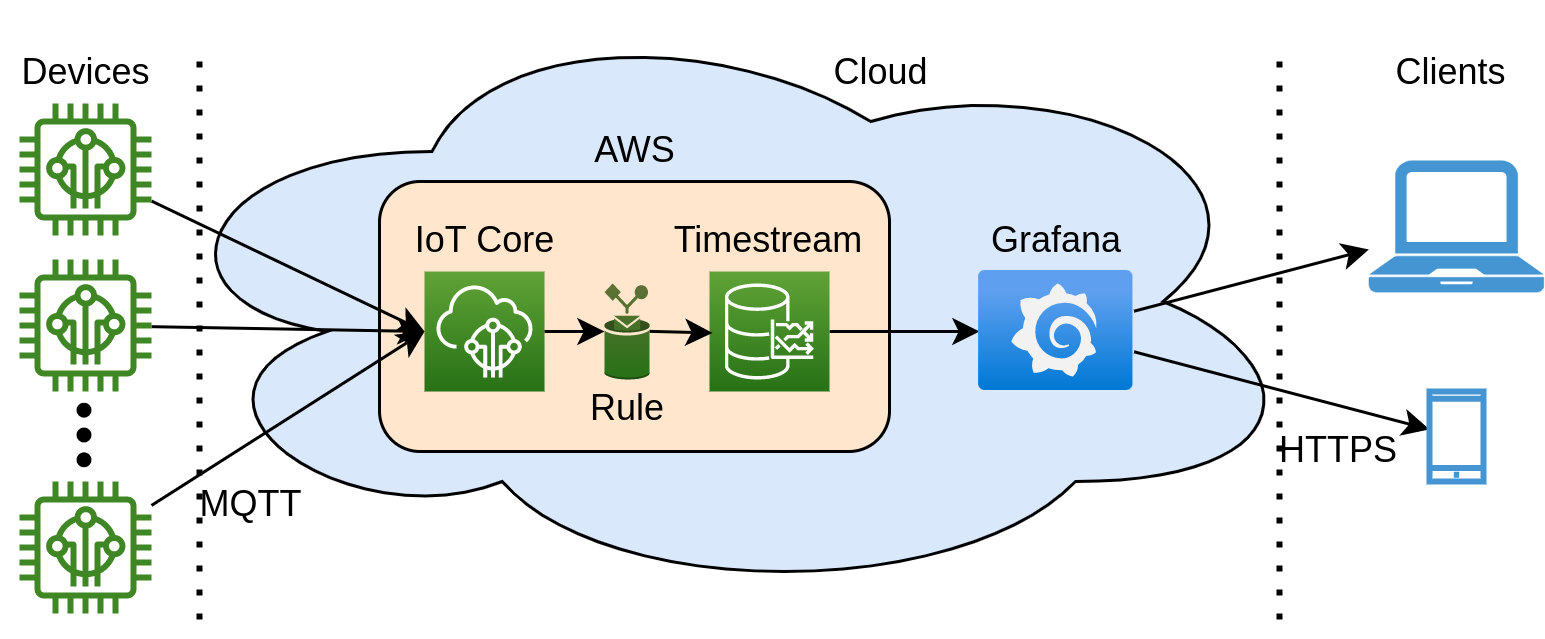
\includegraphics[scale=0.22]{./Figures/cc_diagram.png}
	\caption{Arquitectura de los servicios en la nube.}
	\label{fig:cc_diagram}
\end{figure}

De la figura \ref{fig:cc_diagram} se infiere que los datos generados por los dispositivos son transmitidos por MQTT hacia IoT Core, donde mediante un \textit{rule} se extrae la información relevante y se guarda en una base de datos de Timestream. Los datos de Timestream son utilizados para crear un \textit{dashboard} en Grafana, que puede ser accedido por los clientes a través de un navegador web y el protocolo HTTPS.

\subsection{Gestión de dispositivos con IoT Core}
\label{subsection3_3_1}
Para que los dispositivos se conecten a IoT Core para recibir y transmitir mensajes deben ser previamente registrados. El proceso de registro consistió de los siguientes pasos:

\begin{enumerate}
	\item Crear un \textit{thing}: un \textit{thing} representa el dispositivo físico o virtual que se desea registrar. Se puede crear manualmente a través de la consola de administración de AWS.
	\item Generar certificados y llaves: para habilitar la comunicación segura entre el dispositivo y IoT Core, se deben generar certificados y llaves de seguridad.
	\item Descargar certificados y claves: una vez generados los certificados y llaves, IoT Core proporcionará los archivos necesarios para autenticar y establecer una conexión segura entre el dispositivo y el servicio. Estos archivos incluyen un certificado X.509 \cite{x509_info} del dispositivo, una llave privada y un certificado de autoridad raíz.
	\item Adjuntar políticas de acceso al certificado: el certificado del dispositivo debe ser adjuntado a una determinada política de acceso para que el dispositivo pueda interactuar con los servicios de AWS requeridos.
\end{enumerate}

Todos estos pasos pueden realizarse manualmente a través de la consola web de AWS, pero no resulta un proceso adecuado cuando se desea registrar muchos dispositivos. En cambio, para este trabajo se creó un \textit{script} que utiliza la interface por línea de comandos AWS (aws-cli) \cite{awscli_info} para automatizar esta tarea. En el código \ref{cod:bash_script} se puede observar el código de este \textit{script}.

\begin{lstlisting}[language=bash, label=cod:bash_script, caption=\textit{Script} para automatizar el registro de un dispositivo en AWS IoT Core]
#!/bin/bash

# Create thing, device certificate and private key
AWS_IOT_ENDPOINT="xxxxxxxxxxxxxx-ats.iot.us-east-1.amazonaws.com"
THING_NAME=$(uuidgen)

aws iot create-thing --thing-name $THING_NAME

CERT_ARN=$(aws iot create-keys-and-certificate --set-as-active --certificate-pem-outfile device.pem.crt --private-key-outfile private.pem.key --query 'certificateArn' --output text)

# Attach certificate to thing and policy to certificate
aws iot attach-thing-principal --thing-name $THING_NAME --principal $CERT_ARN
aws iot attach-principal-policy --principal $THING_NAME --principal $CERT_ARN --policy-name IOT_ACCESS

# Update the NVS settings file
NVS_CONFIG="nvs.csv"

awk -v new_value="$THING_NAME" -F ',' '
BEGIN { OFS = FS }
{
  if ($1 == "device_id") {
    $4 = new_value
  }
  print
}
' "$NVS_CONFIG" > "${NVS_CONFIG}.tmp" && mv "${NVS_CONFIG}.tmp" "$NVS_CONFIG"
\end{lstlisting}

La política de acceso asociada al certificado del dispositivo le da permisos para conectarse, publicar, suscribirse y recibir. En el código \ref{cod:policie_json} se muestra la política de acceso en formato JSON.

\begin{lstlisting}[label=cod:policie_json,caption=Politica de acceso asociada a los certificados de los dispositivos.]
{
  "Version": "2012-10-17",
  "Statement": [
    {
      "Effect": "Allow",
      "Action": [
        "iot:Connect",
        "iot:Publish",
        "iot:Subscribe",
        "iot:Receive"
      ],
      "Resource": [
        "*"
      ]
    }
  ]
}
\end{lstlisting}

Para grabar en la memoria del dispositivo los certificados y llaves generados anteriormente, además de otros datos de importancia, se utiliza el generador de particiones NVS incluido en ESP-IDF. Este requiere un archivo de tipo \texttt{.csv} de donde obtiene toda la información que servirá para generar un archivo binario que deberá ser grabado en la región de memoria correspondiente a la partición NVS. En los códigos \ref{cod:nvs_file} y \ref{cod:gen_part} se muestran el archivo \texttt{nvs.csv} y el comando para generar el archivo binario de la partición, respectivamente.

\begin{lstlisting}[label=cod:nvs_file,caption=Archivo nvs.csv.]
key,type,encoding,value    
certs,namespace,,  
dev_id,data,string,abddeab5-3428-4129-bbaf-dab22e15d978
dev_cert,file,string,certificate.pem.crt
priv_key,file,string,private.pem.key
\end{lstlisting}

\begin{lstlisting}[label=cod:gen_part,caption=Comando para crear una particion con el generador de particiones NVS]
nvs_partition_gen.py generate "nvs.csv" nvs.bin 16384
\end{lstlisting}

\subsection{Bases de datos de series temporales con Timestream}
Para almacenar los datos de relevancia que los dispositivos conectados a IoT Core pueden generar, se utilizó Timestream, de esta forma pueden ser accedidos por otros servicios para su posterior procesamiento y visualización. Los pasos que se siguieron para implementar Timestream fueron:

\begin{enumerate}
	\item Crear una base de datos de Timestream: se creó una base de datos con el nombre \texttt{iot} con las opciones que se muestran en la captura de pantalla de la figura \ref{fig:cc_ts_opt}
	\begin{figure}[h]
		\centering
		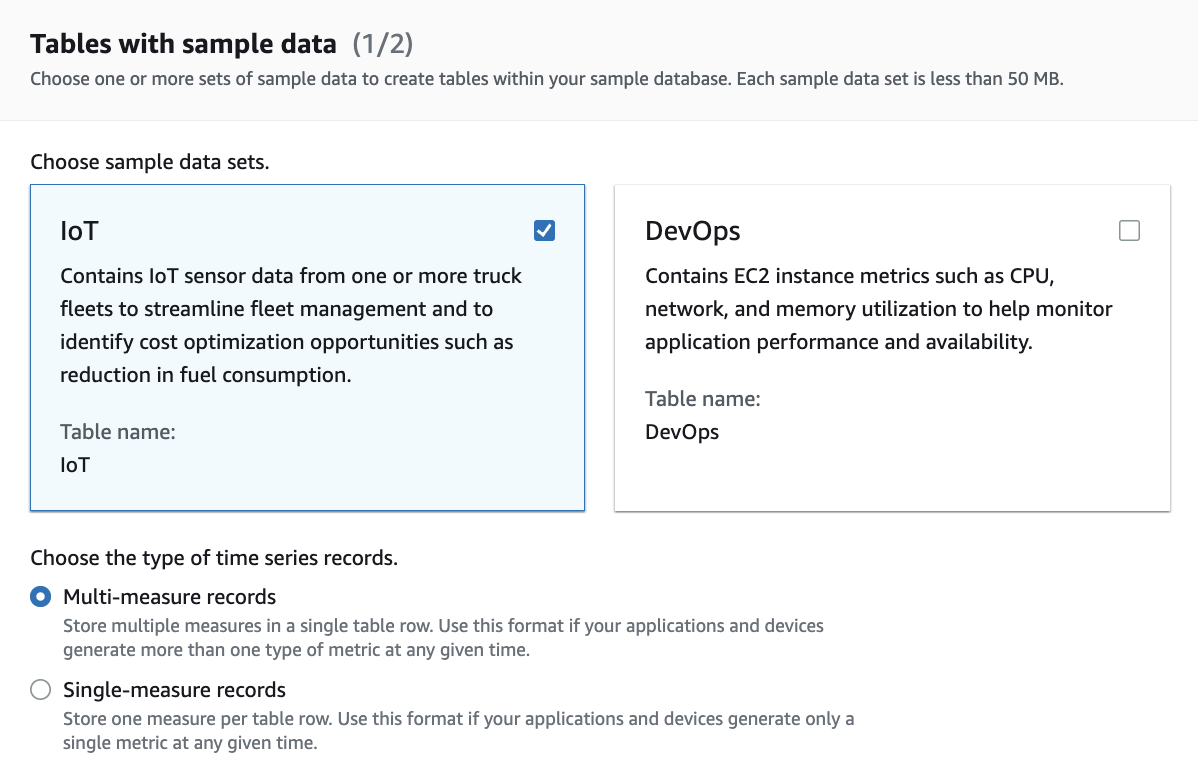
\includegraphics[scale=0.5]{./Figures/cc_ts_opt.png}
		\caption{Captura de pantalla de la creación de una base de datos en Timestream.}
		\label{fig:cc_ts_opt}
	\end{figure}
	
	\item Crear una tabla: dentro de la base de datos \texttt{iot}, se creó una tabla de nombre \texttt{faceCounter} para organizar los datos de series temporales de los dispositivos. En la figura \ref{fig:cc_ts_table} se muestran las opciones para la creación de la tabla \texttt{faceCounter}.
	\begin{figure}[h]
		\centering
		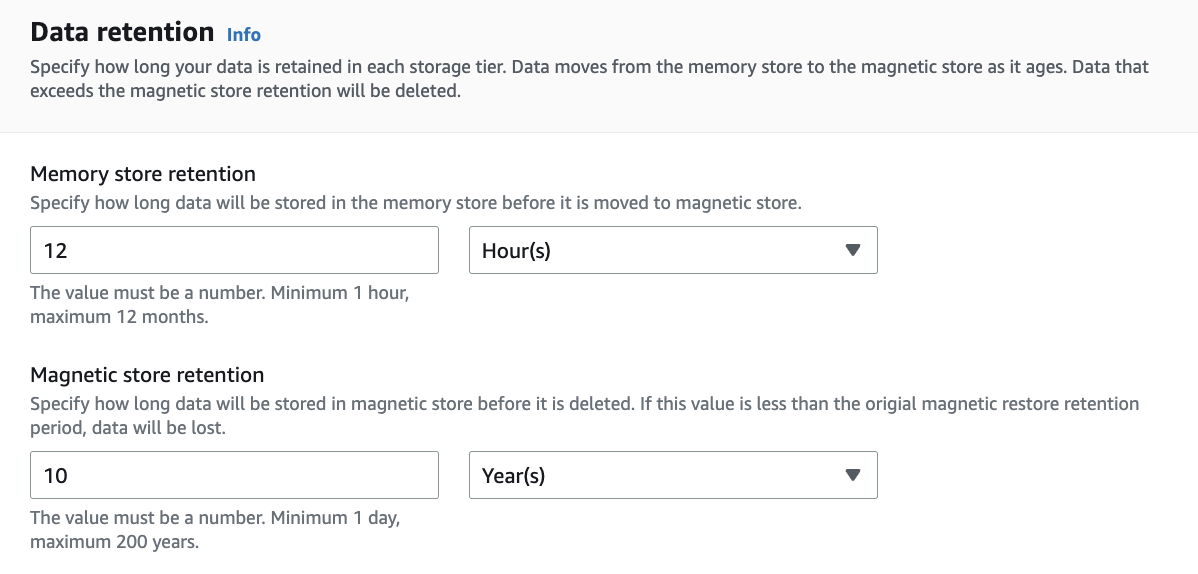
\includegraphics[scale=0.5]{./Figures/cc_ts_table.png}
		\caption{Captura de pantalla de la creación de una tabla en Timestream.}
		\label{fig:cc_ts_table}
	\end{figure}
	
	\item Ingesta de datos: para enviar datos a Timestream se creó un \textit{rule} en IoT Core que redirige los datos relevantes contenidos en los mensajes que llegan al \textit{broker} MQTT hacia la tabla \textit{faceCounter} de la base de datos \textit{iot}. En el código \ref{cod:rule_sql} se muestra el código SQL necesario para extraer los datos que debe ser almacenados en la base de datos.
\begin{lstlisting}[language=SQL, label=cod:rule_sql,caption=Código SQL del \textit{rule} para alcenar datos en Timestream.]
SELECT payload.face AS face, payload.battery AS battery, payload.temperature AS temperature FROM 'faceCounter/data_in'
\end{lstlisting}	
	
\end{enumerate}

\subsection{Visualiación de datos con Grafana}
Una vez creada la base de datos de series temporales para almacenar los datos del dispositivo, puede ser utilizada para ofrecer sus datos a otros servicios, en este caso Grafana. Grafana ofrece integración con Timestream a través del uso de \textit{plugins} y credenciales de acceso a AWS, donde los datos almacenados pueden ser accedidos con el uso del lenguaje SQL. Para visualizar datos con Grafana se deben generar \textit{dashboards} que, a través de elementos de visualización que resultan comprensibles para los usuarios finales. El \textit{dashboard} creado está compuesto por 2 elementos de visualización: 1 gráfico de series de tiempo para los datos de rostros detectados, junto con 2 gráficos indicadores para los datos de estado de la batería y temperatura del dispositivo. En la figura \ref{fig:gr_dashboard} se muestra el \textit{dashboard} creado para este trabajo, mientras que en el código \ref{cod:grafana_sql} se encuentra el código SQL para obtener los datos sobre los rostros detectados de Timestream.

\begin{figure}[h]
	\centering
	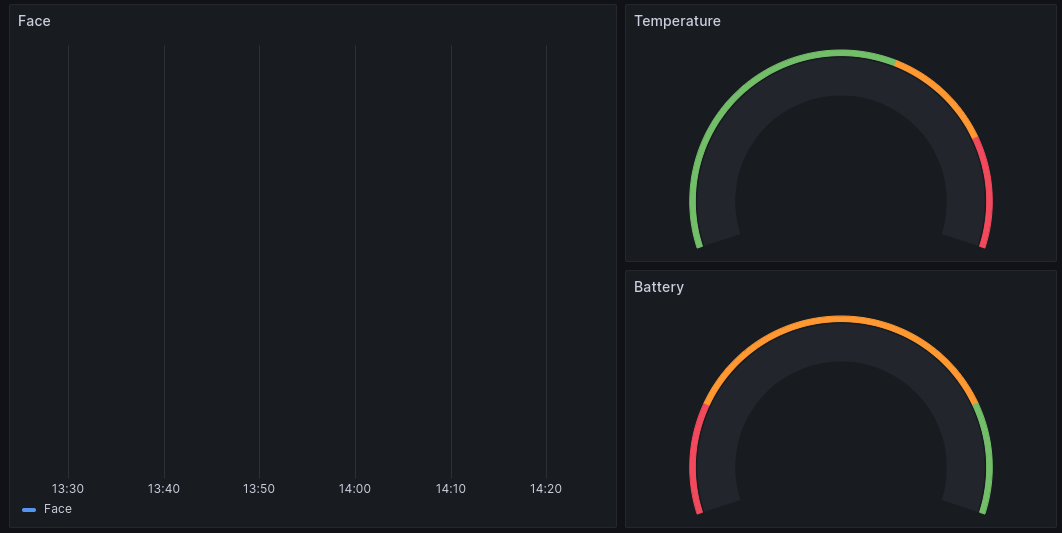
\includegraphics[scale=0.35]{./Figures/cc_dashboard.png}
	\caption{Captura de pantalla del \textit{dashboard}.}
	\label{fig:gr_dashboard}
\end{figure}

\begin{lstlisting}[language=SQL, label=cod:grafana_sql,caption=Código SQL para obtener datos de Tiemstream en Grafana.]
SELECT CREATE_TIME_SERIES(time, measure_value::bigint) as Face
FROM "iot"."mse_test_table" WHERE $__timeFilter
  and measure_name = 'face'
  and device_id = '${id}'
\end{lstlisting}